% Chapter 1

\chapter{Implementation and Data} % Main chapter title

\label{Chapter4} % For referencing the chapter elsewhere, use \ref{Chapter1} 

\lhead{Chapter 4. \emph{Implementation and Data}} % This is for the header on each page - perhaps a shortened title

\emph{In this chapter we present our work, which centers around 66 cross-validated feature engineering experiments including a baseline evaluation. The work is divided into four components: first, the procurement of HEP training data with which to perform the experiments; then, the extensions made to GROBID to facilitate our feature engineering and evaluations; next, the pipeline assembled for automating the experimentation; and finally, the different categories of feature engineering, and our reasons for choosing them.}

\section{Objectives}

As articulated in Chapter \ref{Chapter3}, GROBID manages a hierarchy of models that propagates classified information from top to bottom in a cascade. Our objectives are therefore to enhance some models within the cascade for HEP papers. It does not, on the other hand, make sense to attempt to improve all models. After all, we may assume a HEP \emph{date} is no different from dates printed in other scientific papers. Aside for feature engineering, it is hard to imagine improving performance of these models which exemplary. The same goes for names, and with little exception\footnote{It is in fact true that HEP collaborations feature in isolated references in HEP papers (see Section \ref{sec:futurework}).}, reference lists and their contents. Undoubtedly, the models with the most promising scope for improvement are the \emph{header} and \emph{segmentation} models. It is these models that address the parts of an article most distinct in HEP papers. In particular, some physical journals have recurrent styles and formats for headers sections that are distinct from others publishers. In addition, the vocabularly of a physics headers will be distinct from that papers from other branches of sceience. These should be trained for and additionally engineered for, for example through the use of dictionary-based features (see Section \ref{sec:dicts}). Thus, the \emph{header} model may be improved for a number of reasons, including:

\begin{enumerate}
\item physics publishers present a unique format not found in CORA papers;
\item scientific collaborations as seen in HEP papers are not modelled as a header class by vanilla GROBID, and;
\item discontinuous header data (see Figure XXX), which may contain substantial front matter is by default neither trained nor modelled for.
\end{enumerate}

The \emph{segmentation} model may also be improved for a number of reasons:

\begin{enumerate}
\item discontinuous header data (see Figure XXX), which may contain substantial information is neither trained nor modelled for;
\item HEP collaborations entail long author lists and affiliation lists, often disjoint from the main header section, which are neither trained nor modelled for, and;
\item the dataset is small (we more than double it in Section \ref{sec:data}).
\end{enumerate}

Note that the \emph{segmentation} model is the parent model of the entire cascade, and therefore any improvement to it will benefit all other models at prediction time. Aside from being the root of the cascade, the \emph{segmentation} model is special in that it models. A comparison is given in Table \ref{table:headervssegmentation}. We are mindful of this distinction as we go about our feature engineering.

\begin{table}[h]
\begin{center}
\begin{tabular}{|c|c|c|}
\hline
Model & Token & Instance \\
\hline
Header & Character string & Header section \\
\hline
Segmentation & Full line & Full document \\
\hline
\end{tabular}
\caption[Comparison of token and instance ]{Evaluation results for reference segmentation}
\label{table:headervssegmentation}
\end{center}
\end{table}

Our focus is therefore on the two models, \emph{header} and \emph{segmentation}. We therefore require two separate training sets of HEP papers, one for each model. Incidentally, both models require that for each [paper we produce a TEI representation and a \emph{raw} file of extracted features, as explained in Section \ref{sec:grobid}.

\section{Data Acquisition}
\label{sec:data}

At the recommendation of an INSPIRE-HEP library curator, we selected a set of articles deemed to be a representative sample of the database. It contains the following varieties of papers:

\begin{enumerate}
\item conference papers (no DOI);
\item conference papers (with DOI);
\item general papers;
\item miscellaneous papers (including non-English language), and;
\item collaboration papers.
\end{enumerate}

This totalled 191 papers\footnote{Originally this numbered in excess of 200, but certain papers could not be parsed by \emph{pdf2xml}.}, however according to our adjudications, we additionally removed articles deemed to be unsuitable for training, such as books. The starting point for generating training data is to apply the existing, default models of GROBID on the new dataset of PDF papers. For \emph{segmentation} training data, the command for this is \texttt{createTrainingSegmentation}. 

In Sections \ref{subsec:cora}, \ref{subsec:hepdatasetheader}, and \ref{subsec:hepdatasetsegmentation}, we detail the mixture of data we have assembled.

\begin{table}[h]
\begin{center}
\begin{tabular}{|c|c|c|}
\hline
Model & HEP & CORA \\
\hline
Header & 157 & \textbf{2506} \\
\hline
Segmentation & \textbf{169} & 125 \\
\hline
\end{tabular}
\caption[Number of training instances for each model from each dataset.]{Number of training instances for each model from each dataset.}
\label{table:headervssegmentation}
\end{center}
\end{table}

\subsection{CORA dataset}
\label{subsec:cora}
The CORA (ACRONYM) dataset is a substantial dataset of some 2506 header instances. It is popular in metadata extraction studies, as creating custom training data is a stupendously time-consuming task, and has come to be a sort of standard (\cite{Peng04accurateinformation}). From One of the questions we ask in Section \ref{sec:results} is therefore, what 

\begin{enumerate}
\item the dataset is small (we more than double it in Section \ref{sec:data})
\item the dataset is small (we more than double it in Section \ref{sec:data})
\item the dataset is small (we more than double it in Section \ref{sec:data})
\item the dataset is small (we more than double it in Section \ref{sec:data})
\end{enumerate}

Despite the overall quality of the dataset, we did encounter some small mistakes, as do (\cite{Peng04accurateinformation})

\blockquote{The \emph{note} field is the one most confused with others, and upon inspection is actually labeled inconsistently in the training data.}

\subsection{HEP dataset - Header}
\label{subsec:hepdatasetheader}

We were therefore able to experiment with combining the two datasets of HEP papers, as well as subsampling the CORA dataset to see . After all, in spite of common wisdom that increasing the amount of training data will increase generalisation and model performance, it is not clear what effects combining different ground truths, namely CORA and HEP, will have. One may imagine that generalising over a hybrid dataset might construct a misleading model when it comes to evaluate on a pure HEP dataset, especially when the CORA set dwarfs our HEP one. Therefore one of our research questions is whether such a mixture is beneficial, and we experiment with different CORA sample sizes in Section \ref{Chapter5}.

\begin{figure}
\centering
\begin{tabular}{cc}
\subfloat[Headnote]{
\includegraphics[width=0.45\textwidth]{Figures/collaboration.pdf}}&
\subfloat[Page number]{
\includegraphics[width=0.45\textwidth]{Figures/eamonn.pdf}} \\
\subfloat[Body (formula)]{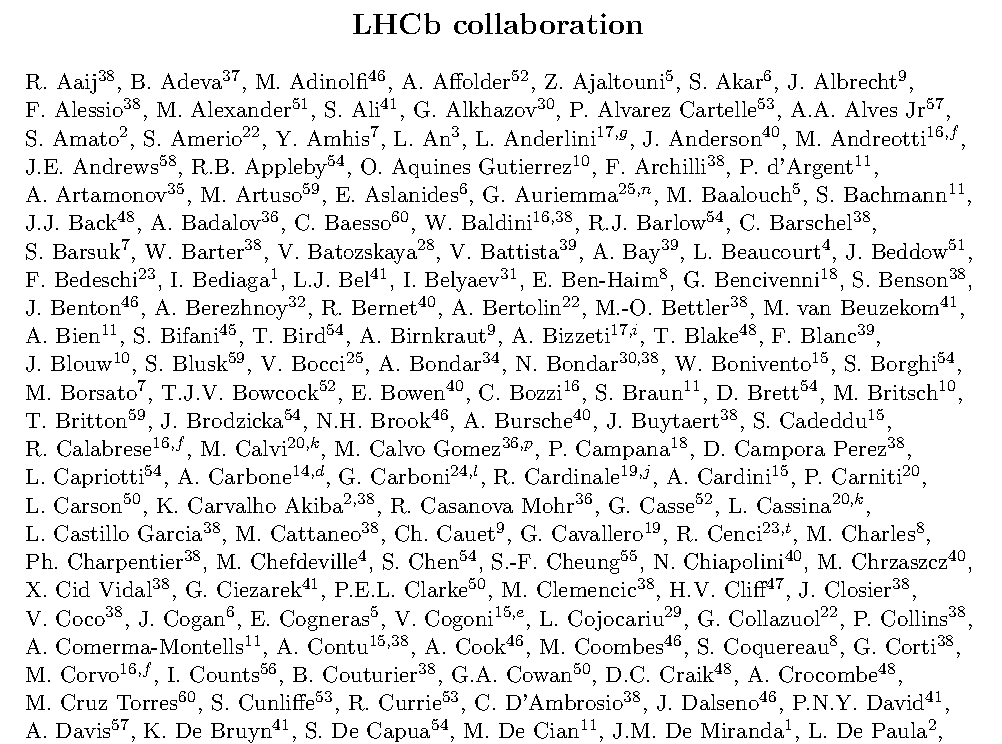
\includegraphics[width=0.45\textwidth]{Figures/authors.pdf}} & 
\subfloat[Body (normal)]{
\includegraphics[width=0.45\textwidth]{Figures/affiliations.pdf}}\\
\end{tabular}
\caption{Discontinuous front matter from (\cite{maguire2012taxonomy}), other excerpts from (\cite{aaij2015identification}).}
\end{figure}

\subsection{HEP dataset - Segmentation}
\label{subsec:hepdatasetsegmentation}

We were therefore able to experiment with combining the two datasets of HEP papers

\section{Extensions}

\begin{enumerate}
\item Confusion matrix
\item k worst files
\item Logging reprts
\item reconnecting header with segmentation model
\end{enumerate}

[INCLUDE SOME CODE HERE]

\section{Pipeline}

Python wrappers for GROBID, k fold cross validation, drawing on python libraries scikit-learn, numpy, matplotlib (pylab) etc.

[INCLUDE SOME CODE HERE]

\section{Feature Engineering}

Here we list the ideas for feature functions that we implemented and cross-validate for (see Section \ref{Chapter5}).

\subsection{Baseline}

Baseline features include token identities, prefixes, suffixes, captilisation etc.

In addition, we examined the effects of ramping up the size of the CORA set appended during training.

\subsection{Dictionaries}
\subsection{Dictionaries + Stops}
\subsection{Regularisation}

We additionally cross-validated the tuning parameter for the model, the variance for $l_2$ normalisation, $\sigma^2$, as . Unlike the true feature engineering work, this involved configuring 

\subsection{Token Extensions}

To allow this, modifications were made to GROBID to allow analysis over the full line.

\subsection{Block Shape}

\subsection{Levenshtein Distance}

\begin{equation}
  \text{lev}_{a, b}(i, j) = 
  \begin{cases} 
  	\text{max}(i, j) &\quad\text{if min(i, j) = 0} \\
	\text{min}
		\begin{cases}
			\text{lev}_{a, b}(i - 1, j) + 1 \\
			\text{lev}_{a, b}(i, j - 1) + 1 \\
			\text{lev}_{a, b}(i - 1, j - 1) + 1_{a_i \neq b_j} \\
		\end{cases} &\quad\text{otherwise} \\
  \end{cases}
\label{eq:levenshtein}
\end{equation}

\begin{equation}
\text{similarity}_{a, b} = 1 - \frac{\text{lev}_{a, b}(|a|, |b|)}{\text{max}(|a|, |b|)}
\label{eq:levenshteinsimilarity}
\end{equation}

\subsection{Character Classes}

A visual scan of any scientific paper allows one to see that lines from different sections are most easily distinguished by the composition of characters. It therefore stands to reason that we can build informative features for the \emph{segmentation} model on this basis. Thus, we see how a line may be more effectively characterised at the \emph{character} level than the \emph{word} level.

Note that the baseline feature function set does include some basic capitalisation and punctuation indicators, but we advocate our approach for several reasons:

\begin{enumerate}
\item it is more complete in that it models more character classes;
\item it does this systematically in a feature framework that is easily modified or extended, and;
\item it performs better (see Chapter \ref{Chapter5}).
\end{enumerate}

\begin{table}[h]
\begin{center}
\begin{tabular}{|c|l|l|}
\hline
Index & Class & Regex\\
\hline
0 & Spacing & \verb|r`[\s]'|\\
1 & Lower case & \verb|r`[a-z]'|\\
2 & Upper case & \verb|r`[A-Z]'|\\
3 & Numeric & \verb|r`[\d]'|\\
4 & Punctuation & \verb|r`[\(\).,?:;]'|\\
5 & Special character & \verb|r`[^\sa-zA-Z\d\(\).,?:;]'|\\
\hline
\end{tabular}
\caption[Character classes used as features, along with the regular expressions used to count them.]{Character classes used as features, along with the regular expressions used to count them.}
\label{table:characterclasses}
\end{center}
\end{table}

\begin{figure}
\centering
\begin{tabular}{cc}
\subfloat[Body (formula)]{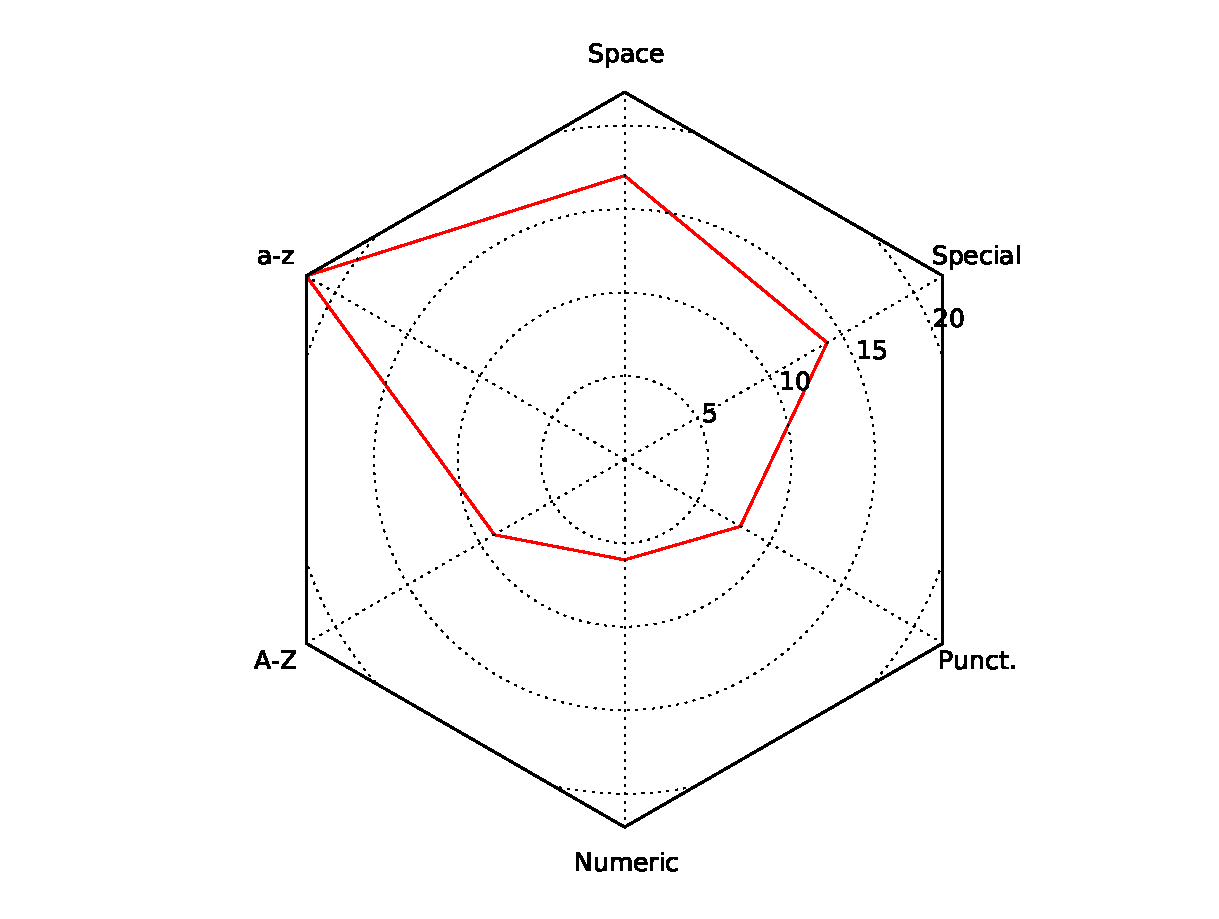
\includegraphics[width=0.5\textwidth]{Figures/body_formula.pdf}} & 
\subfloat[Body (normal)]{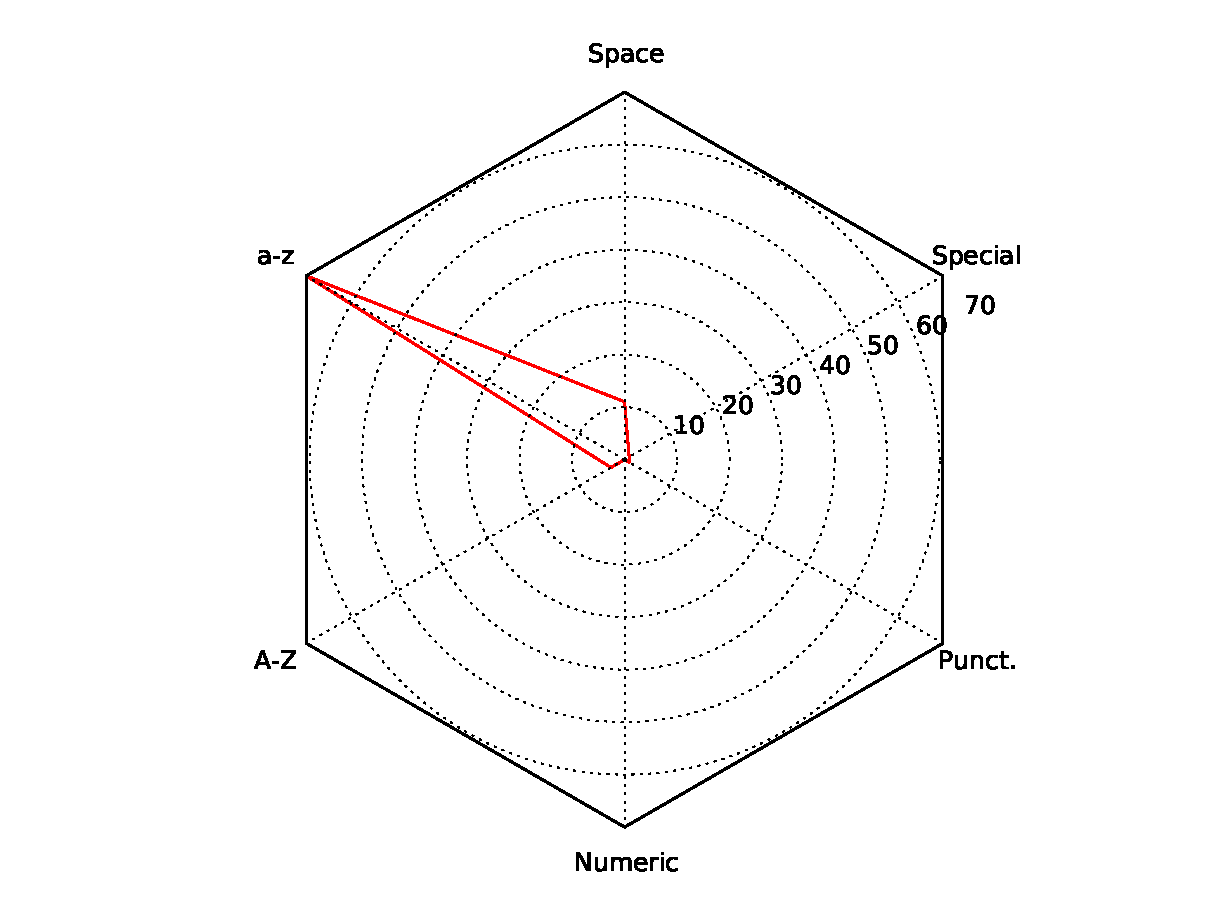
\includegraphics[width=0.5\textwidth]{Figures/body_normal.pdf}}\\
\subfloat[Headnote]{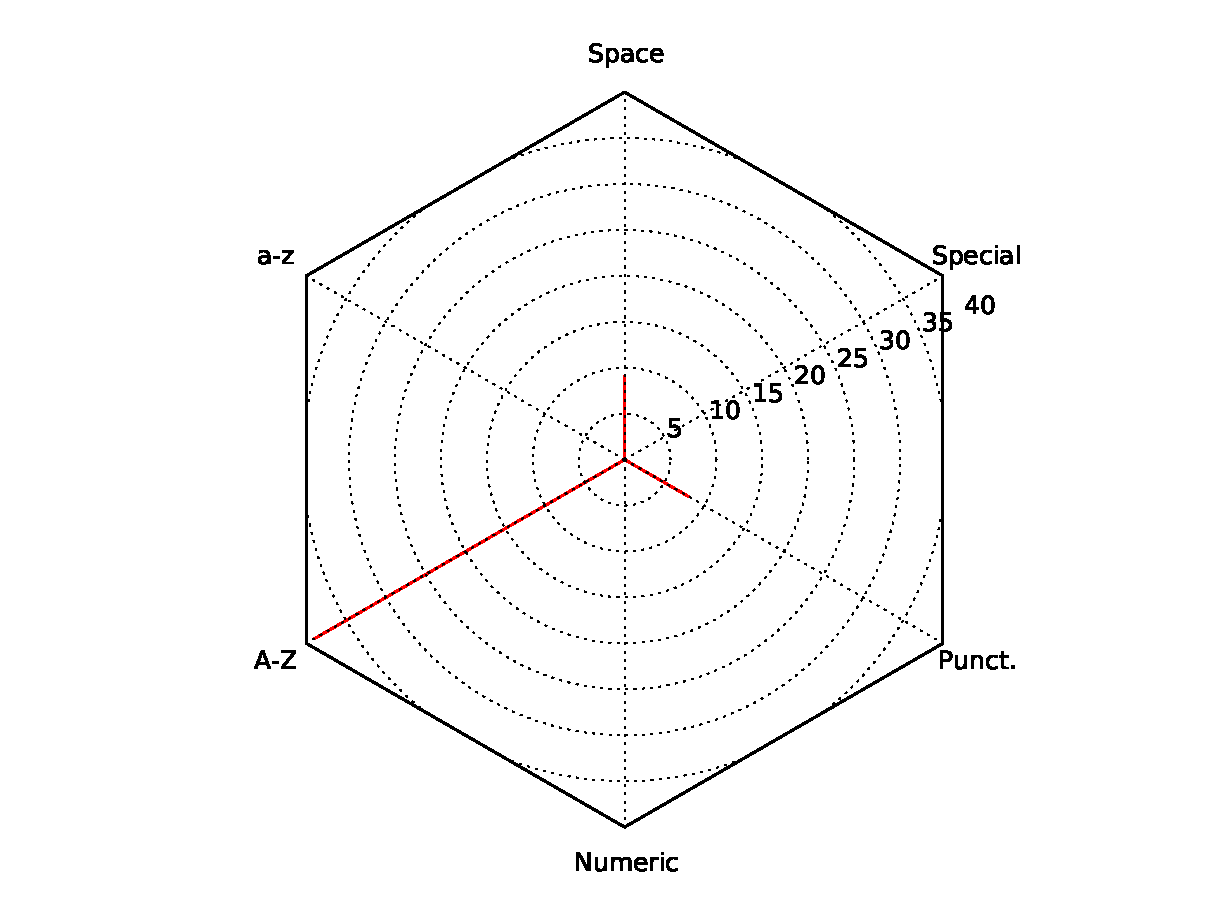
\includegraphics[width=0.5\textwidth]{Figures/headnote.pdf}}&
\subfloat[Page number]{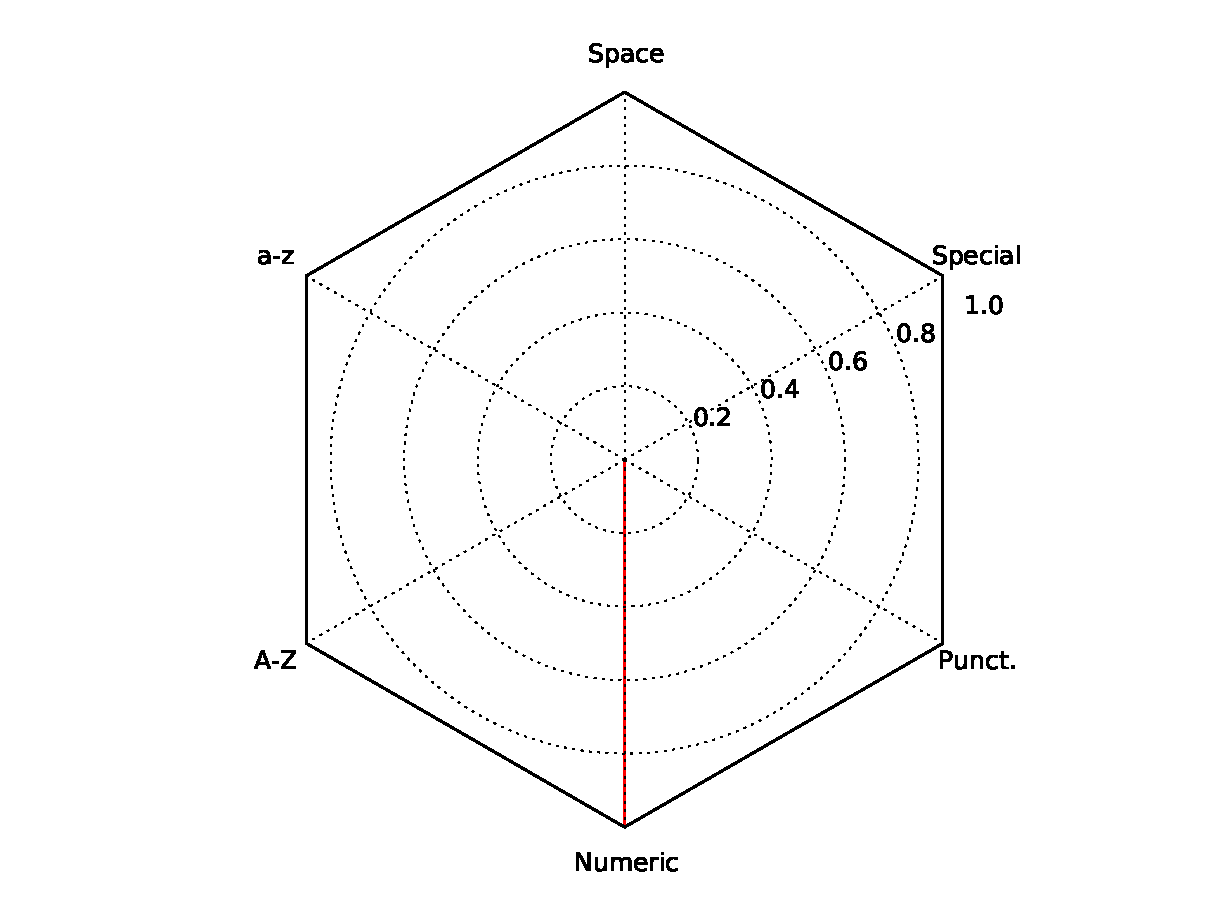
\includegraphics[width=0.5\textwidth]{Figures/page.pdf}} \\
\subfloat[Affilation list]{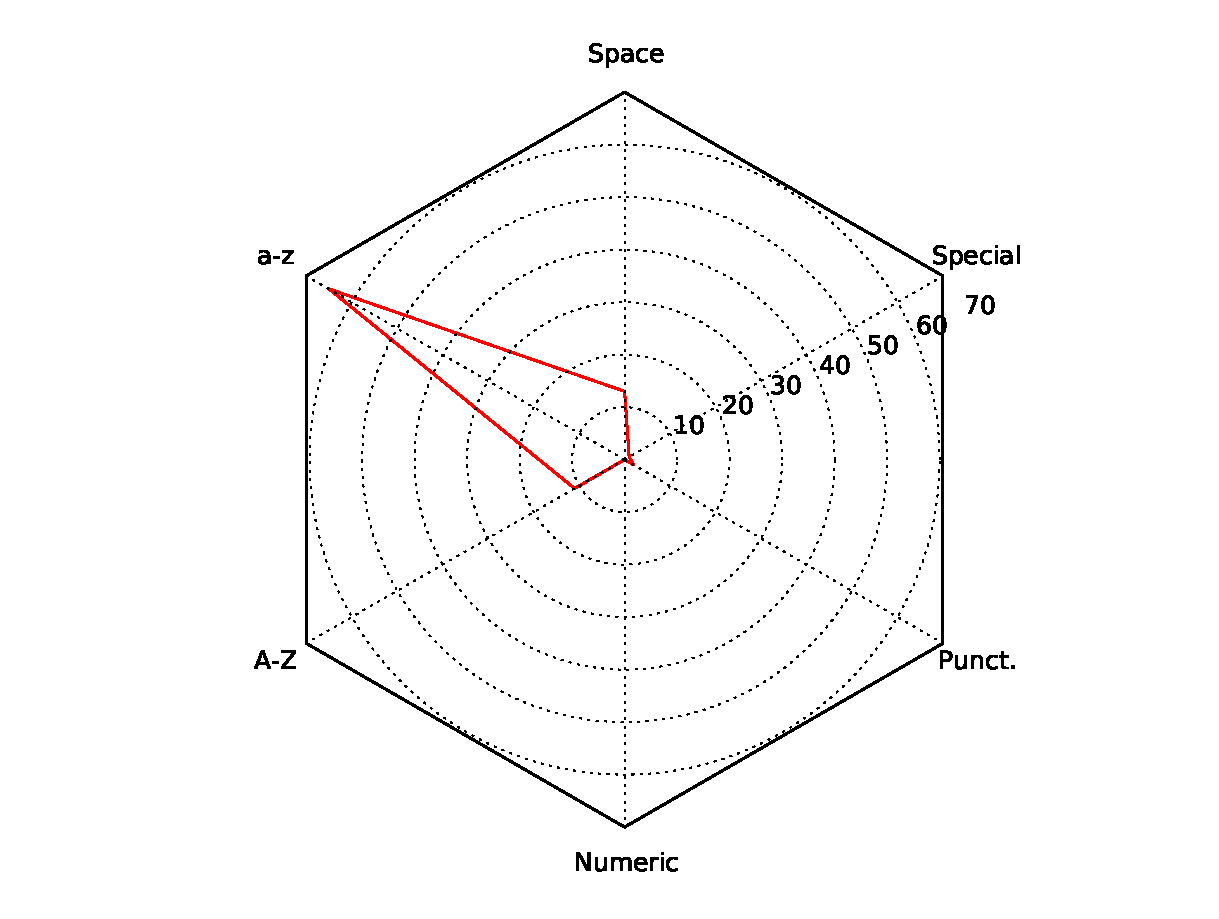
\includegraphics[width=0.5\textwidth]{Figures/affiliations_list.pdf}} & 
\subfloat[Author list]{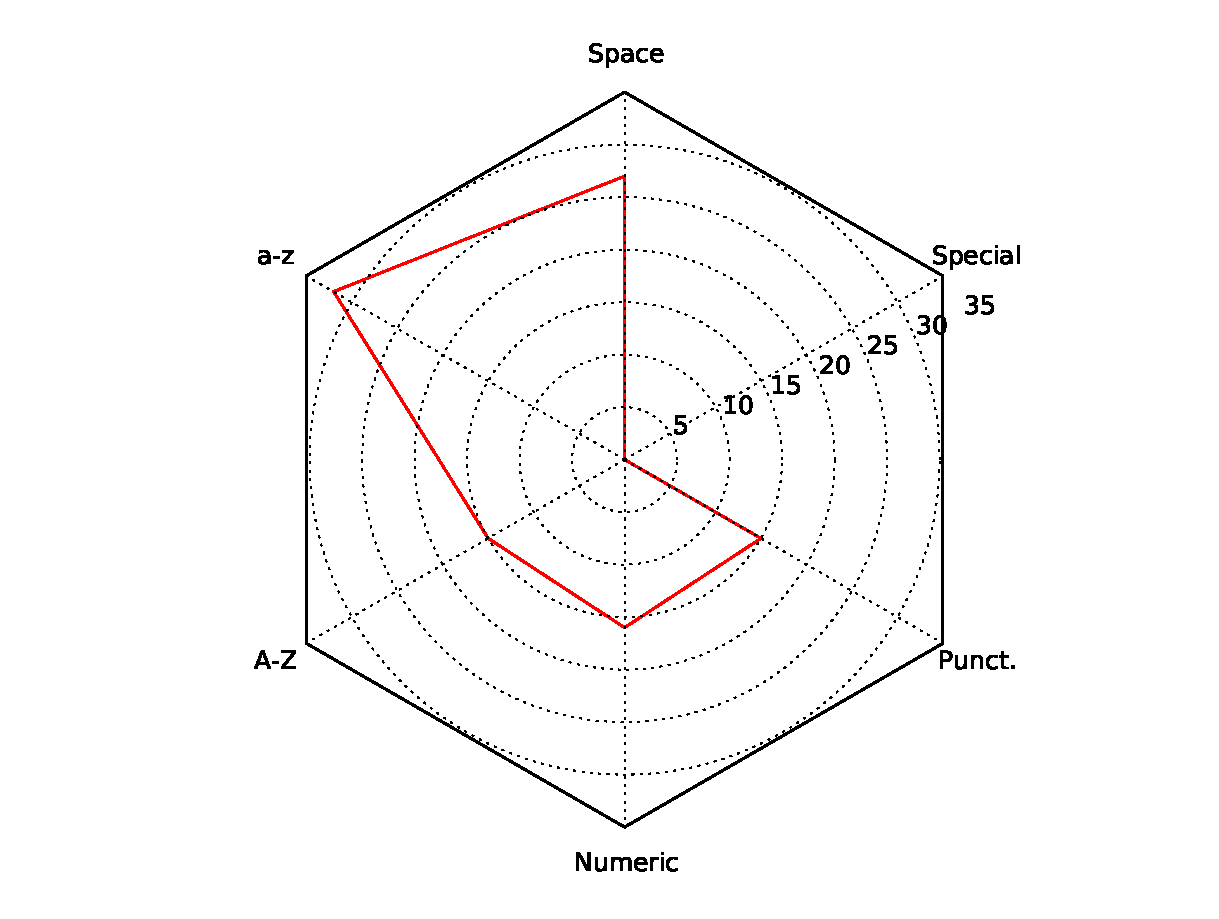
\includegraphics[width=0.5\textwidth]{Figures/author_list.pdf}} \\ 
\end{tabular}
\caption{Character class breakdown of sample lines from different sections of a CERN LHCb collaboration paper. The paper in question is the current world record holder for number of authors, and lists over 5000 authors and their affilations. The radar plots give a different impression for each of the samples.}
\end{figure}
